\documentclass[tikz,border=8pt]{standalone}
\usepackage{amsmath}
\usetikzlibrary{arrows.meta}
\definecolor{ink}{HTML}{21352F}
\definecolor{teal}{HTML}{087F7B}
\definecolor{blue}{HTML}{4B77A8}
\definecolor{gold}{HTML}{C58B2A}
\definecolor{rose}{HTML}{B65A62}
\begin{document}
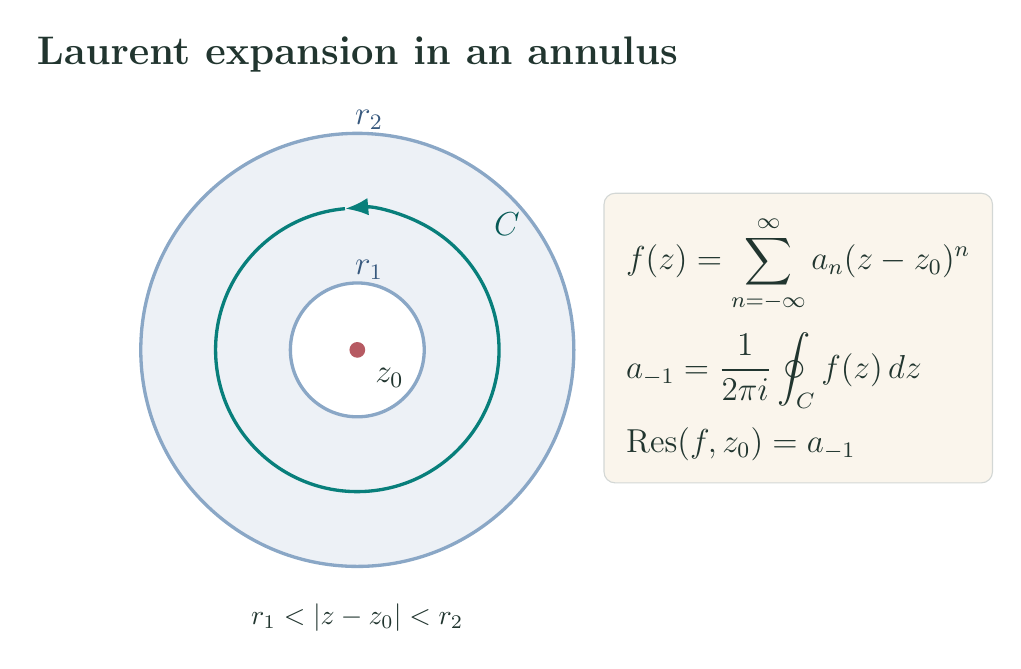
\begin{tikzpicture}[font=\large\sffamily,text=ink,>=Latex]
  \node[font=\bfseries\Large] at (0,3.75)
    {Laurent expansion in an annulus};
  \fill[blue!10,even odd rule] (0,0) circle (2.75) (0,0) circle (.85);
  \draw[blue!65,very thick] (0,0) circle (2.75);
  \draw[blue!65,very thick] (0,0) circle (.85);
  \draw[teal,very thick,->] (1.8,0)
    arc[start angle=0,end angle=95,radius=1.8];
  \draw[teal,very thick] ({1.8*cos(95)},{1.8*sin(95)})
    arc[start angle=95,end angle=360,radius=1.8];
  \fill[rose] (0,0) circle (.1);
  \node[below right=3pt] at (0,0) {$z_0$};
  \node[blue!75!black] at (.15,1.02) {$r_1$};
  \node[blue!75!black] at (.15,2.92) {$r_2$};
  \node[teal!70!black] at (1.9,1.6) {$C$};
  \node[draw=ink!20,fill=gold!9,rounded corners=4pt,
        inner sep=8pt,align=left] at (5.6,.15)
    {$\displaystyle
      f(z)=\sum_{n=-\infty}^{\infty}a_n(z-z_0)^n$\\[6pt]
     $\displaystyle
      a_{-1}=\frac1{2\pi i}\oint_Cf(z)\,dz$\\[6pt]
     $\displaystyle
      \operatorname{Res}(f,z_0)=a_{-1}$};
  \node[font=\normalsize] at (0,-3.4)
    {$r_1<|z-z_0|<r_2$};
\end{tikzpicture}
\end{document}
